%----------------------------------------------------------------------------------------
%    PACKAGES AND THEMES
%----------------------------------------------------------------------------------------
\documentclass[aspectratio=169,xcolor=dvipsnames]{beamer}
\makeatletter
\def\input@path{{../BeamerTemplate/theme/}}
\makeatother
\usetheme{CleanEasy}
\usepackage[utf8]{inputenc}
\usepackage{lmodern}
\usepackage[T1]{fontenc}
\usepackage{fix-cm}
\usepackage{amsmath}
\usepackage{mathtools}
\usepackage{listings}
\usepackage{xcolor}
\usepackage{hyperref}
\usepackage{graphicx}
\usepackage{booktabs}
\usepackage{tikz}
\usetikzlibrary{positioning, shapes, arrows, calc, decorations.pathreplacing, arrows.meta, backgrounds, patterns, overlay-beamer-styles}
\usepackage{etoolbox}
\usepackage{animate}

%----------------------------------------------------------------------------------------
%    LAYOUT CONFIGURATION
%----------------------------------------------------------------------------------------
\input{../BeamerTemplate/configs/configs}

%----------------------------------------------------------------------------------------
%    TITLE PAGE CONFIGURATION
%----------------------------------------------------------------------------------------
\title[Stacks]{Data Structures: Stacks}
\author{Data Structure Course}
\institute{DGIST}
\date{\today}

% Simple title page without logos
\titlegraphic{}

%----------------------------------------------------------------------------------------

\begin{document}

\begin{frame}[plain]
  \titlepage
\end{frame}

\begin{frame}[plain]{Contents}
  \tableofcontents
\end{frame}

%----------------------------------------------------------------------------------------
%    INTRODUCTION
%----------------------------------------------------------------------------------------
\section{Introduction to Stacks}

\begin{frame}{What is a Stack?}
  \begin{definition}
    A \textbf{stack} is a linear data structure that follows the \textbf{Last In, First Out (LIFO)} principle.
  \end{definition}
  
  \vspace{0.5cm}
  
  \begin{columns}
    \begin{column}{0.6\textwidth}
      Key characteristics:
      \begin{itemize}
        \item Elements are added and removed from the same end (top)
        \item Only the top element is accessible
        \item Perfect for managing nested operations and histories
        \item Natural structure for function calls and recursion
      \end{itemize}
    \end{column}
    \begin{column}{0.35\textwidth}
      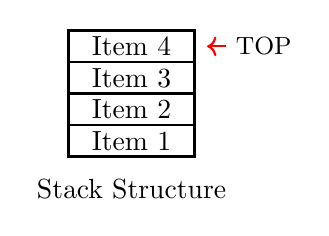
\begin{tikzpicture}[scale=0.8]
        \draw[thick] (0,0) rectangle (2,0.5);
        \draw[thick] (0,0.5) rectangle (2,1);
        \draw[thick] (0,1) rectangle (2,1.5);
        \draw[thick] (0,1.5) rectangle (2,2);
        
        \node at (1,0.25) {Item 1};
        \node at (1,0.75) {Item 2};
        \node at (1,1.25) {Item 3};
        \node at (1,1.75) {Item 4};
        
        \draw[->, thick, red] (2.5,1.75) -- (2.2,1.75);
        \node[right] at (2.5,1.75) {\small TOP};
        
        \node[below] at (1,-0.2) {Stack Structure};
      \end{tikzpicture}
    \end{column}
  \end{columns}
\end{frame}

%----------------------------------------------------------------------------------------
%    CORE OPERATIONS
%----------------------------------------------------------------------------------------
\section{Core Operations}

\begin{frame}[fragile]{Essential Stack Operations}
  \begin{columns}
    \begin{column}{0.5\textwidth}
      \begin{block}{Primary Operations}
        \begin{itemize}
          \item \textbf{Push}: Add element to top
          \item \textbf{Pop}: Remove and return top element
          \item \textbf{Peek/Top}: Return top element without removing
          \item \textbf{Empty}: Check if stack is empty
          \item \textbf{Size}: Get number of elements
        \end{itemize}
      \end{block}
    \end{column}
    \begin{column}{0.45\textwidth}
      \begin{exampleblock}{C Example}
        \begin{lstlisting}[language=C,basicstyle=\tiny\ttfamily]
int s[100];
int top = -1;          // empty

// push
s[++top] = 10;
s[++top] = 20;

// peek (top element)
int topVal = s[top];   // -> 20

// pop
int x = s[top--];      // -> 20

// empty?
int empty = (top == -1);
        \end{lstlisting}
      \end{exampleblock}
    \end{column}
  \end{columns}
  
  \vspace{0.5cm}
  
  \begin{alertblock}{Time Complexity}
    All operations are \textbf{O(1)} - constant time (amortized for push in dynamic arrays)
  \end{alertblock}
\end{frame}

\begin{frame}{Stack Operations Visualization}
  \begin{center}
    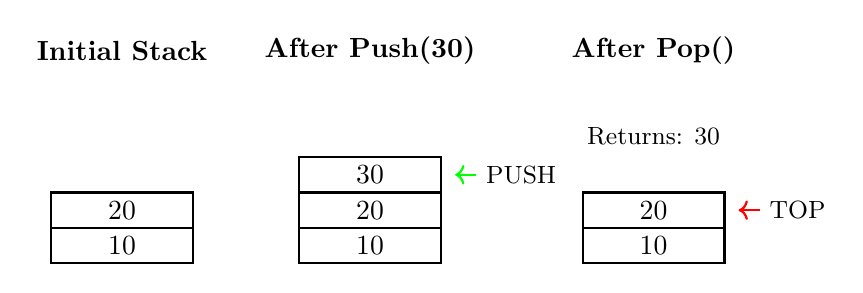
\begin{tikzpicture}[scale=0.9]
      % Initial stack
      \node at (1,3) {\textbf{Initial Stack}};
      \draw[thick] (0,0) rectangle (2,0.5);
      \draw[thick] (0,0.5) rectangle (2,1);
      \node at (1,0.25) {10};
      \node at (1,0.75) {20};
      
      % Push operation
      \node at (4.5,3) {\textbf{After Push(30)}};
      \draw[thick] (3.5,0) rectangle (5.5,0.5);
      \draw[thick] (3.5,0.5) rectangle (5.5,1);
      \draw[thick] (3.5,1) rectangle (5.5,1.5);
      \node at (4.5,0.25) {10};
      \node at (4.5,0.75) {20};
      \node at (4.5,1.25) {30};
      \draw[->, thick, green] (6,1.25) -- (5.7,1.25);
      \node[right] at (6,1.25) {\small PUSH};
      
      % Pop operation
      \node at (8.5,3) {\textbf{After Pop()}};
      \draw[thick] (7.5,0) rectangle (9.5,0.5);
      \draw[thick] (7.5,0.5) rectangle (9.5,1);
      \node at (8.5,0.25) {10};
      \node at (8.5,0.75) {20};
      \draw[->, thick, red] (10,0.75) -- (9.7,0.75);
      \node[right] at (10,0.75) {\small TOP};
      
      \node at (8.5,1.8) {\small Returns: 30};
    \end{tikzpicture}
  \end{center}
\end{frame}

%----------------------------------------------------------------------------------------
%    IMPLEMENTATIONS
%----------------------------------------------------------------------------------------
\section{Implementation Approaches}

\begin{frame}{Array-based vs Linked List Implementation}
  \begin{columns}
    \begin{column}{0.48\textwidth}
      \begin{block}{Array-based Stack}
        \textbf{Pros:}
        \begin{itemize}
          \item Contiguous memory
          \item Great cache locality
          \item Simple implementation
          \item O(1) amortized push
        \end{itemize}
        
        \textbf{Cons:}
        \begin{itemize}
          \item Occasional resize cost
          \item Capacity management
        \end{itemize}
      \end{block}
    \end{column}
    \begin{column}{0.48\textwidth}
      \begin{block}{Linked List-based Stack}
        \textbf{Pros:}
        \begin{itemize}
          \item No resize cost
          \item Always O(1) operations
          \item Dynamic size
        \end{itemize}
        
        \textbf{Cons:}
        \begin{itemize}
          \item Extra pointer memory
          \item Poor cache locality
          \item More complex
        \end{itemize}
      \end{block}
    \end{column}
  \end{columns}
\end{frame}

\begin{frame}[fragile]{Linked List Stack Implementation}
  \begin{lstlisting}[language=Python,basicstyle=\small\ttfamily]
class Node:
    def __init__(self, val, next=None):
        self.val = val
        self.next = next

class StackLL:
    def __init__(self):
        self.head = None
        self.n = 0

    def push(self, x):
        self.head = Node(x, self.head)
        self.n += 1

    def pop(self):
        if not self.head:
            raise IndexError("pop from empty stack")
        x = self.head.val
        self.head = self.head.next
        self.n -= 1
        return x

    def peek(self):
        if not self.head:
            raise IndexError("peek from empty stack")
        return self.head.val
  \end{lstlisting}
\end{frame}

%----------------------------------------------------------------------------------------
%    APPLICATIONS
%----------------------------------------------------------------------------------------
\section{Applications}

\begin{frame}[fragile]{Expression Evaluation: Parentheses Matching}
  \begin{exampleblock}{Problem}
    Check if parentheses, brackets, and braces are properly balanced.
  \end{exampleblock}
  
  \begin{columns}
    \begin{column}{0.45\textwidth}
      \textbf{Algorithm:}
      \begin{enumerate}
        \item Push opening brackets onto stack
        \item For closing brackets:
          \begin{itemize}
            \item Check if stack is empty
            \item Check if top matches type
            \item Pop if match, return false if not
          \end{itemize}
        \item Stack should be empty at end
      \end{enumerate}
    \end{column}
    \begin{column}{0.5\textwidth}
      \begin{lstlisting}[language=Python,basicstyle=\tiny\ttfamily]
def valid_brackets(s):
    pairs = {')':'(', ']':'[', '}':'{'}
    st = []
    for ch in s:
        if ch in '([{':
            st.append(ch)
        elif ch in ')]}':
            if not st or st[-1] != pairs[ch]:
                return False
            st.pop()
    return not st

# Examples:
# valid_brackets("([]){}") -> True
# valid_brackets("([)]") -> False
      \end{lstlisting}
    \end{column}
  \end{columns}
\end{frame}

\begin{frame}{Function Call Stack and Recursion}
  \begin{columns}
    \begin{column}{0.55\textwidth}
      \begin{block}{Call Stack Mechanism}
        \begin{itemize}
          \item Each function call creates a \textbf{stack frame}
          \item Frame contains: parameters, local variables, return address
          \item Recursion uses call stack implicitly
          \item Deep recursion can cause stack overflow
        \end{itemize}
      \end{block}
      
      \begin{alertblock}{Converting Recursion to Iteration}
        Use explicit stack to avoid stack overflow for deep recursion
      \end{alertblock}
    \end{column}
    \begin{column}{0.4\textwidth}
      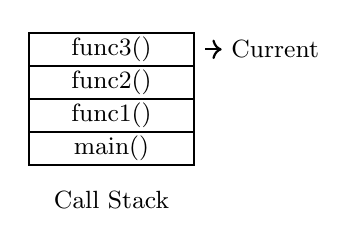
\begin{tikzpicture}[scale=0.7]
        \draw[thick] (0,0) rectangle (3,0.6);
        \draw[thick] (0,0.6) rectangle (3,1.2);
        \draw[thick] (0,1.2) rectangle (3,1.8);
        \draw[thick] (0,1.8) rectangle (3,2.4);
        
        \node at (1.5,0.3) {\small main()};
        \node at (1.5,0.9) {\small func1()};
        \node at (1.5,1.5) {\small func2()};
        \node at (1.5,2.1) {\small func3()};
        
        \draw[->, thick] (3.2,2.1) -- (3.5,2.1);
        \node[right] at (3.5,2.1) {\small Current};
        
        \node[below] at (1.5,-0.3) {\small Call Stack};
      \end{tikzpicture}
    \end{column}
  \end{columns}
\end{frame}

\begin{frame}{Undo/Redo Operations}
  \begin{columns}
    \begin{column}{0.5\textwidth}
      \begin{block}{Two-Stack Approach}
        \begin{itemize}
          \item \textbf{Undo Stack}: stores performed actions
          \item \textbf{Redo Stack}: stores undone actions
        \end{itemize}
      \end{block}
      
      \textbf{Operations:}
      \begin{itemize}
        \item \textbf{Action}: push to undo, clear redo
        \item \textbf{Undo}: pop from undo, apply inverse, push to redo
        \item \textbf{Redo}: pop from redo, apply, push to undo
      \end{itemize}
    \end{column}
    \begin{column}{0.45\textwidth}
      Simple undo/redo pattern in pseudocode:
      \begin{itemize}
        \item \texttt{do(action)} - execute and save
        \item \texttt{undo()} - reverse last action
        \item \texttt{redo()} - replay undone action
      \end{itemize}
    \end{column}
  \end{columns}
  
  \vspace{0.3cm}
  \begin{exampleblock}{Real-world Examples}
    Text editors, image editing software, IDEs, web browsers
  \end{exampleblock}
\end{frame}

%----------------------------------------------------------------------------------------
%    COMPLEXITY ANALYSIS
%----------------------------------------------------------------------------------------
\section{Complexity Analysis}

\begin{frame}{Time and Space Complexity}
  \begin{center}
    \begin{tabular}{l|c|c|c}
      \toprule
      \textbf{Implementation} & \textbf{Push} & \textbf{Pop/Peek} & \textbf{Space} \\
      \midrule
      Array-based & O(1) amortized & O(1) & O(n) \\
      Linked List-based & O(1) & O(1) & O(n) + pointer overhead \\
      \bottomrule
    \end{tabular}
  \end{center}
  
  \vspace{0.5cm}
  
  \begin{columns}
    \begin{column}{0.48\textwidth}
      \begin{block}{Array-based Considerations}
        \begin{itemize}
          \item Amortized O(1) push due to resize
          \item Worst-case single push: O(n)
          \item Better cache performance
        \end{itemize}
      \end{block}
    \end{column}
    \begin{column}{0.48\textwidth}
      \begin{block}{Linked List Considerations}
        \begin{itemize}
          \item Guaranteed O(1) for all operations
          \item Extra memory per node
          \item Dynamic allocation overhead
        \end{itemize}
      \end{block}
    \end{column}
  \end{columns}
\end{frame}

%----------------------------------------------------------------------------------------
%    CONCLUSION
%----------------------------------------------------------------------------------------
\section{Summary}

\begin{frame}{Key Takeaways}
  \begin{block}{Stack Fundamentals}
    \begin{itemize}
      \item LIFO data structure with top-only access
      \item Essential operations: push, pop, peek, empty, size
      \item All operations are O(1) time complexity
    \end{itemize}
  \end{block}
  
  \begin{block}{Implementation Choices}
    \begin{itemize}
      \item Array-based: better cache, amortized O(1)
      \item Linked list-based: guaranteed O(1), more memory
    \end{itemize}
  \end{block}
  
  \begin{block}{Important Applications}
    \begin{itemize}
      \item Expression evaluation and parentheses matching
      \item Function call management and recursion
      \item Undo/redo functionality
      \item Backtracking algorithms
      \item Converting recursive to iterative algorithms
    \end{itemize}
  \end{block}
\end{frame}

\begin{frame}[plain]
  \begin{center}
    {\Huge Thank You!}
    
    \vspace{1cm}
    
    {\large Questions?}
  \end{center}
\end{frame}

\end{document}